

\subsection{PDSurvey Platform}

	The public display survey (\textit{PDSurvey}) platform aims to facilitate the conduction and evaluation of surveys on and for public displays. 
		% We developed this platform with the aim for ...
	The interactive survey platform, which can be embedded directly onto public displays and be used as a direct feedback channel from inside another application, can be split into three main parts: PDAdmin, PDServer, and PDClient (see Figure \ref{fig:4-pdsurvey-platform}). \textit{PDAdmin} contains the administrative interface, allowing display providers to configure questionnaires for their public displays. \textit{PDServer} accommodates the REST service, the persistence layer, and the majority of the application logic. \textit{PDClient} is a web based interface, containing one possibility for responding to the deployed surveys. 

	The code base of all three parts is deliberately separated from each other, allowing the independent refinement and less dependencies between the frontend, the backend, and the server.

	% The \textit{PDSurvey} platform can be split into three main sections:



	\begin{figure}%[btph]
	    \begin{center}
	        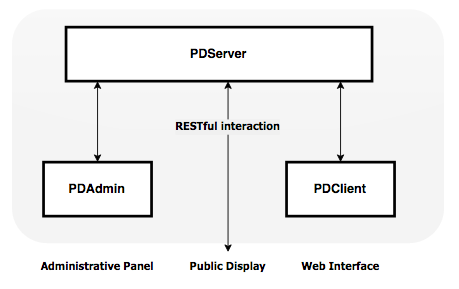
\includegraphics[width=.7\columnwidth]{img/4_implementation/4-overview}
	    \end{center}
	 \caption[Overview of the PDSurvey platform]{Overview of the PDSurvey platform: (a) PDServer containing the Node.js server, (b) PDBackend is the entry point for administrators and (c) PDClient the interface included on public displays and optimized for mobile devices.}
	 \label{fig:4-pdsurvey-platform}
	\end{figure}




	\subsubsection{PDAdmin}

		For administrative purposes we created an admin interface, enabling display providers to create, manage and distribute surveys to public displays. 		Display providers have the ability to create their own questionnaires or to select from a list of standardized questionnaires (introduced in section \ref{sec:questionnaires}).

		The entry point for PDAdmin is the dashboard. There a user gets an overview of information such as how their campaigns are running, and how many responses have been submitted already. 
		% Wizard
		For new users who haven't created any campaigns, questionnaires or displays yet, get prompted to use the Getting Started wizard (see figure \ref{}).

		% normal process

			% SCREENSHOTS from WIZARD

			

		% detail views of each panel
			% A displays
			% B surveys
			% C campaigns


		% TODO add Screenshots

			% SCREENSHOT: Wizard
			% SCREENSHOT: individually accessing 1 Display / 2 Surveys / 3 Campaigns
			% SCREENSHOT: Dashboard

	\subsubsection{PDServer}

		PDServer makes a relatively simple impression. It consists of a Node.js server, which to the outside only acts as a REST server. Processing REST calls, performing CRUD operations and responding with JSON objects. Besides this REST functionality a rudimentary authentication mechanism is already implemented on the server and the capability for further logic, determining which client should ask which question next. This functionality might become of interest when trying to spread standardized questionnaires of longer length across multiple users or multiple displays. It would be intended for the server to keep track which questions have already been answered and to tell each instance of PDClient which question to ask next, in order to achieve a balanced question profile.

		% Mongoose maintians the object models and performs all CRUD applications on MongoDB 
		%  >> don't get too technical!!

		The specification of PDServer's REST API can be found in the documentation (see Appendix \ref{appendix:documentation}).



	\subsubsection{PDClient}

		Our client tool was kept as simple and minimalistic as possible. It is running on a separated code base than PDBackend, the only communication between the two is via REST, exchanging JSON objects. Reasons for this were on the one hand reduction of the application size, on the other hand different requirements for constructing a PDAdmin interface for a limited number of users, compared with PDClient, being embedded at large scale.

		% TODO: maybe move this paragraph to Section "Implementation: PDClient"
		The goal is to reduce logic and complexity on client-side. Currently PDClient is implemented as follows: The client either receives all questions for the questionnaire (caching the questions), or it loads just the next question on-demand. For this purpose the REST interface provides the /nextQuestion API is provided. For production use one sub-page per campaign gets created, individualized via the campaign ID.
		

		% Overview of elements
		PDClient has three main components (see figure \ref{fig:4-pdsurvey-platform}). The principal part being the \textit{Survey page}. All questions are loaded at once on initial startup, then one question gets displayed at a time. Settings for the survey can be modified in the PDBackend (e.g. number of questions to display and duration of the survey). Once the user makes a choice, it is directly logged on the server. In case that a participant aborts answering the survey, the questions answered so far are still recorded. The \textit{About page} was added, since employees from university gave feedback to us regarding the public display installation, prior to the beginning of development for the PDSurvey platform. They said they were skeptical and had doubts regarding the research project, when having no information whatsoever regarding which information is logged. To motivate people to participate, a \textit{Welcome page} was added. It turned out that a significant larger number of people were willing to participate in a survey, after knowing that it doesn't take long, the research is university-related and that it will be used for a Master's thesis. These arguments were amongst others stated in semi-structured interviews, carried out as part of the field study (see chapter \ref{chapter:field-study}).


		% TODO EMBED SCREENSHOTS HERE!!
		% \begin{figure}%[btph]
		%     \begin{center}
		%         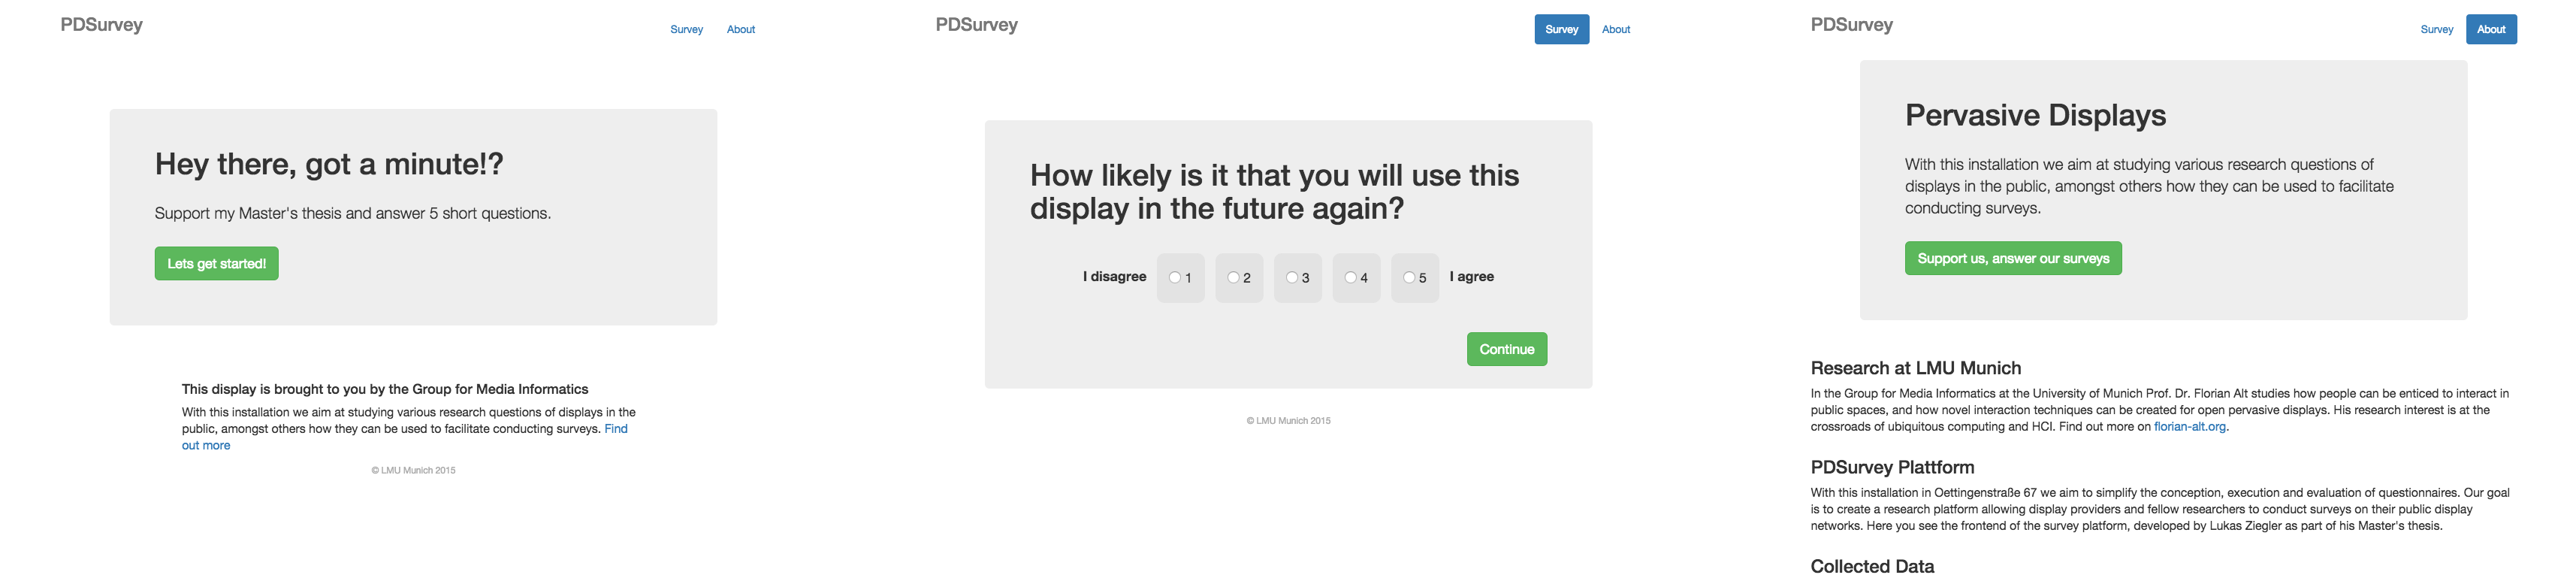
\includegraphics[width=\columnwidth]{img/screenshots/pdclient-overview}
		%     \end{center}
		% 	\caption[Overview of PDClient]{PDClient: (a) Welcome Page, (b) Survey page, (c) About page}
		%  \label{fig:4-pdclient-screenshots}
		% \end{figure}



		\begin{figure}
		    \centering
		    \begin{subfigure}[b]{0.6\textwidth}
		        \centering
		        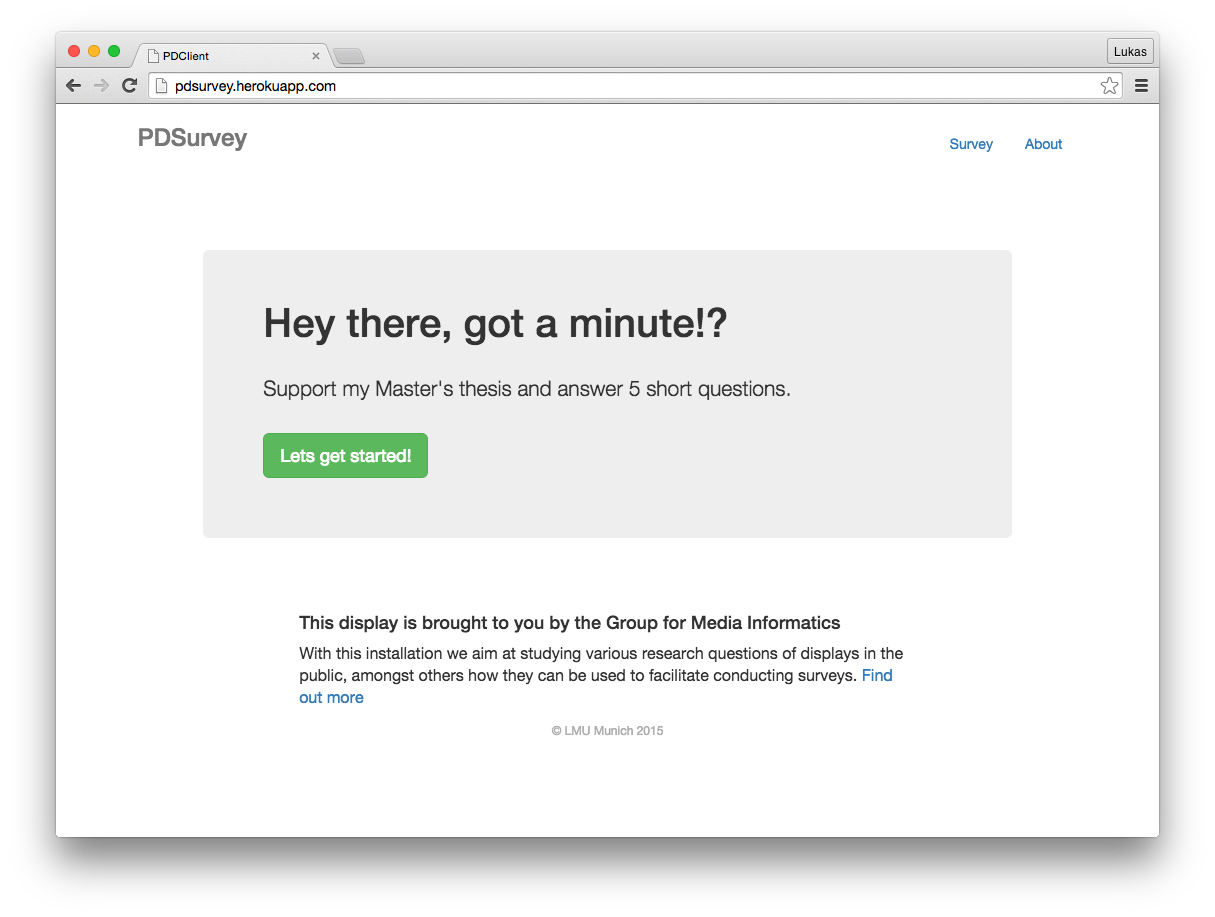
\includegraphics[width=\textwidth]{img/screenshots/pdclient/welcome}
		        \caption{Welcome Page}
		        \label{fig:4-pdclient-welcome}
		    \end{subfigure}
		    \hfill
		    \begin{subfigure}[b]{0.6\textwidth}
		        \centering
		        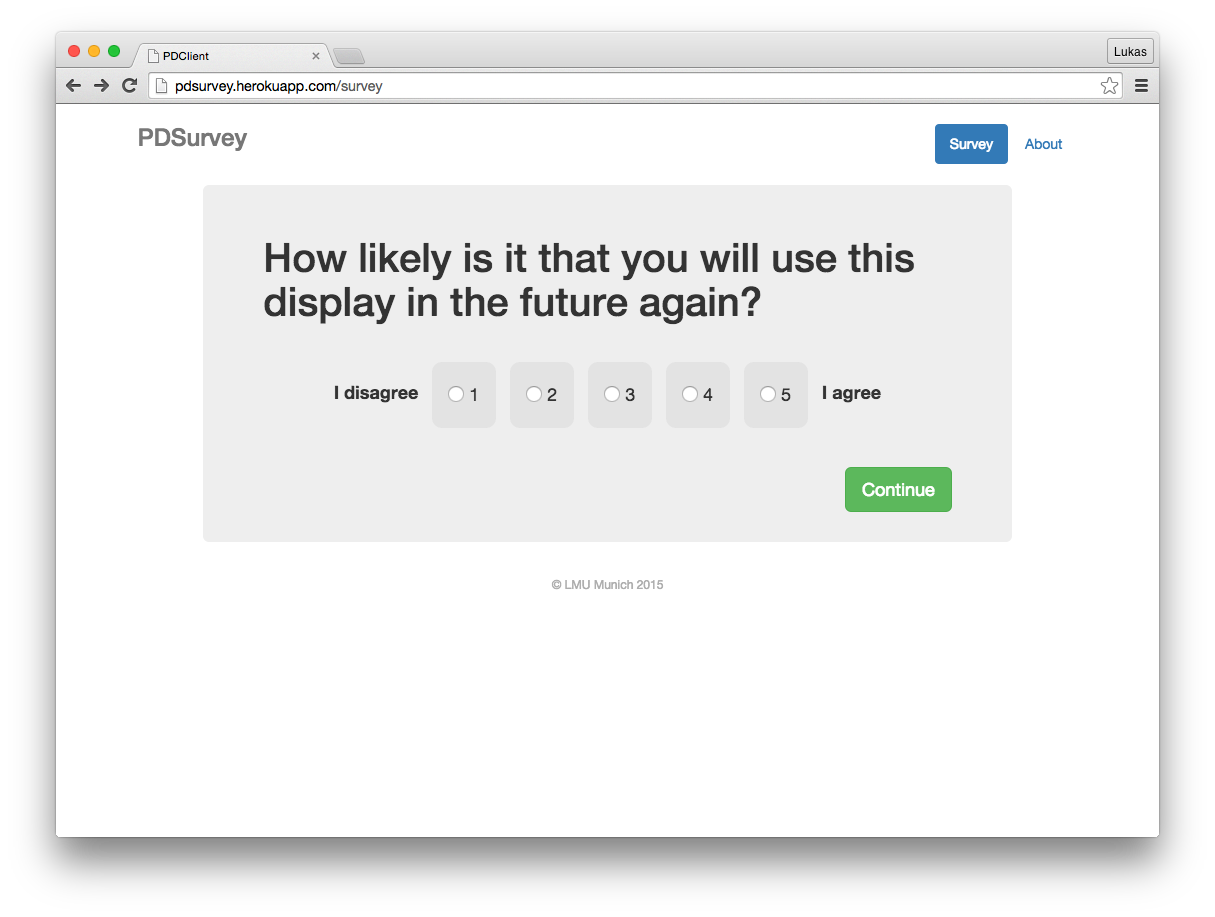
\includegraphics[width=\textwidth]{img/screenshots/pdclient/survey}
		        \caption{Survey page}
		        \label{fig:4-pdclient-survey}
		    \end{subfigure}
		    \hfill
		    \begin{subfigure}[b]{0.6\textwidth}
		        \centering
		        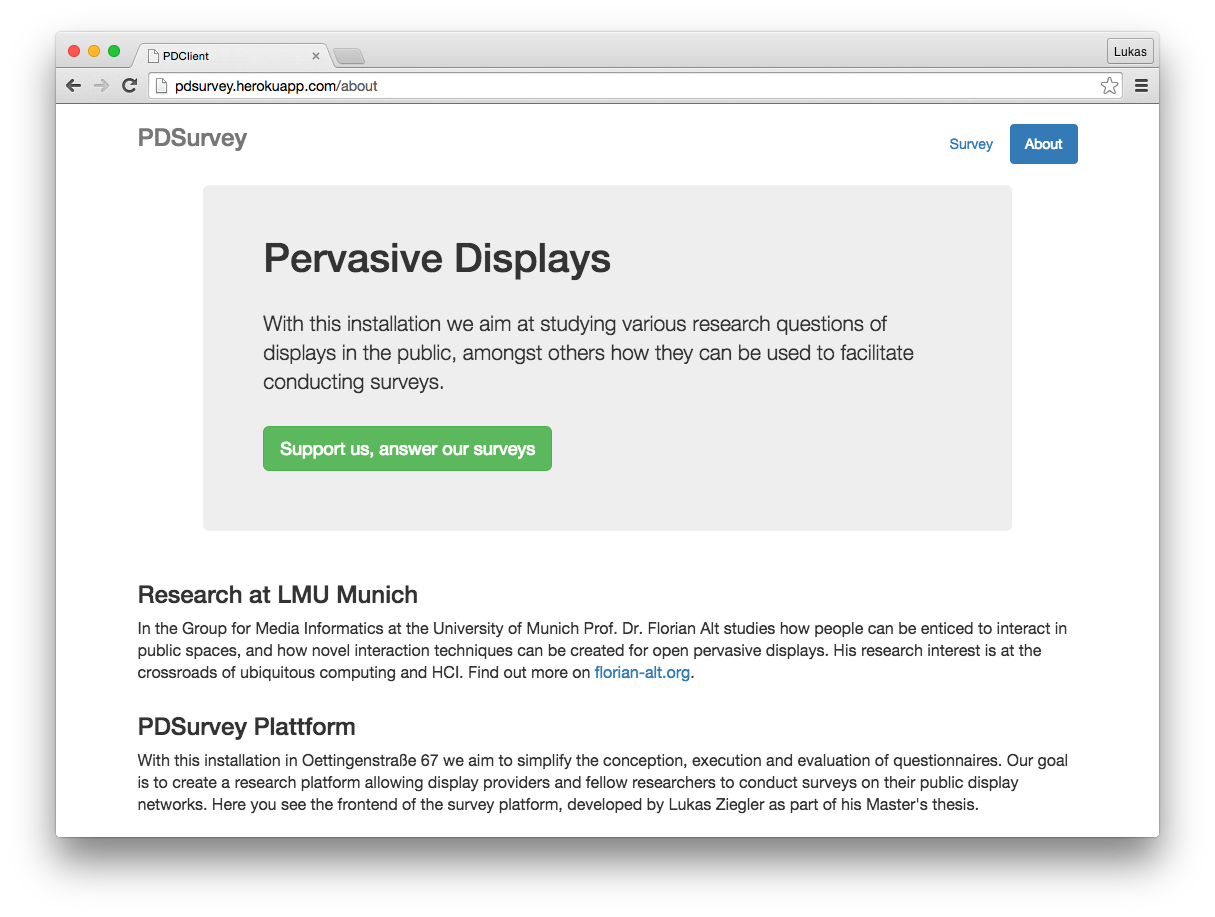
\includegraphics[width=\textwidth]{img/screenshots/pdclient/about}
		        \caption{About page}
		        \label{fig:4-pdclient-about}
		    \end{subfigure}
		    \caption{Overview of PDClient}
		    \label{fig:pdclient-screenshots}
		\end{figure}



	\subsubsection{EmbedCode}

		The embed code, JavaScript Code Injection, turned out to be a pure proof-of-concept, since it was not needed for the field study at the university. The problem was that the application on which PDSurvey should be integrated did not support any HTTP calls, thus we had to fall back on another solution. This embed code was intended to be used by display operators, wanting to include optional questionnaires hovering over their normal application. 

		% also show the mockup / technical demonstration of the JavaScript embed code. It was a proof-of-concept, demonstrating the feasibility of embedding questionnaires as an overlay (additional DIV layer), injected via one (minified) line of Javascript. 

		% Use Case
		An example use case is exemplified here ... \textbf{TODO TODO TODO}
			% -Solutions: (pdsurvey/public/tracking/survey.js bzw. testing/tracking-code/index.html)
		


		% Implementation
		The implementation is quite simple. A JavaScript code snippet will be given to the display provider, which has to be added before the closing body-tag. This minified line of JavaScript code adds a HTML <script>-tag to the DOM of the HTML page, injecting a remote JavaScript file from the PDSurvey platform. This personalized scripts first loads jQuery and/or Angular.js asynchronously, and thereafter creates another instance of the PDClient on client side, inside of the primary website DOM. All questions for the questionnaire get loaded via REST API from the server and the responses get sent back to the server for logging.

		% order to create an overlay with questionnaires (see Figure \textbf{... TODO TODO TODO ...}).

		One important aspect is to prefix all classes and files with a unique namespace, to prevent any sort of collisions with the main program, where the code gets injected into. For this prototype all CSS Bootstrap classes were prefixed with $pd-$.

		Useful links for the development of this prototype were Google Analytics concept of tracking\footnote{\url{https://developers.google.com/analytics/resources/concepts/gaConceptsTrackingOverview} (last visited on November 26, 2014)}, Wikipedia describing the Web Bug \footnote{\url{http://en.wikipedia.org/wiki/Web_bug} (last visited on November 26, 2014)}, and a Stackoverflow discussion regarding embed codes \footnote{\url{http://stackoverflow.com/questions/3534524/how-does-the-embedded-google-analytics-javascript-work} (last visited on November 26, 2014)}.

		For inspiration, of what the finished embed code functionality could have looked like, have a look at the Qualtrics blog article ``Website Feedback Surveys''\footnote{\url{http://www.qualtrics.com/site-intercept/website-feedback/} (last visited on April 6, 2015)} and at the demo of Qualtrics Site Intercept.



	\subsubsection{Feedback Channels}

	As of now PDSurvey offers a ready built survey tool for all devices being capable of running a browser and displaying the PDClient website. Thus a large number of feedback channels is conceivable. For our scenario these were a tablet, smartphone, and laptop/desktop. Integrating PDClient on a public display itself is also no problem, as long as the public display application is a web application itself (embed code), or it supports embedding a browser window on top of the application. 

	In case that the application does not integrate well with a web page being displayed on top of the actual application, then a custom integration needs to be built making use of the REST calls. All REST calls needed to receive the questionnaire and send responses to the PDSurvey platform (in JSON format) can be found in the documentation (see Appendix \ref{appendix:documentation}).



	\subsubsection{(Future Work)}

		PROBABLY PUT THIS IN THE VERY END OF THE PLATFORM; BEFORE CONCLUSION

		% what is still missing

		Authentication: using passport, HTTPS was not offered in the beginning. As of now it is not needed, since we only had one client. All REST Update and Delete functionality was restricted to the URI of the PDServer, which is also the desired approach in the production setting.

		Evaluation of results: dynamic queries, information visualization

		Context: refine the Context model and build the evaluation of the responses based on the Context model, assigned to each and every display and/or campaign.

		Unit testing: not done yet

